\documentclass{mirea}

\institution{Институт искусственного интеллекта}
\faculty    {Кафедра общей информатики}
\worktype   {ОТЧЕТ \\ ПО ПРАКТИЧЕСКОЙ РАБОТЕ №8}
\workname   {Реализация заданной логической функции от четырех переменных на мультиплексорах 16-1, 8-1, 4-1, 2-1}
\subject    {ИНФОРМАТИКА}
\author     {Краснов Н.O.}
\examiner   {Павлова Е.С.}

\usepackage{microtype}
\usepackage{graphicx}	
\usepackage{tikz}
\usetikzlibrary{tikzmark,decorations.pathreplacing}

\begin{document}

\chapter{ПОСТАНОВКА ЗАДАЧИ}
В соответствии с вариантом, в формуле (\ref{eq:Ориг. формула}) дана логическая функция от четырех переменных, заданная в шестнадцатеричной форме:
\begin{equation} \label{eq:Ориг. формула}
	F(a,b,c,d)=E8DD
\end{equation}

Восстановим таблицу истинности. По таблице истинности реализуем в лабораторном комплексе логическую функцию на мультиплексорах следующими способами:

\begin{itemize}
	\item используя один мультиплексор 16-1;
	\item используя один мультиплексор 8-1;
	\item используя минимальное количество мультиплексоров 4-1;
	\item используя минимальную комбинацию мультиплексоров 4-1 и 2-1;
\end{itemize}

Протестируем работу схем и убедимся в правильности их работы.

\chapter{ПРОЕКТИРОВАНИЕ И РЕАЛИЗАЦИЯ}
\section{Восстановленная таблица истинности}
Преобразуем записанную выше формулу (\ref{eq:Ориг. формула}) в двоичную запись:
\[1110\ 1000\ 1101\ 1101_{2}\] – получили столбец значений логической функции, который необходим для восстановления полной таблицы истинности (см. табл. \ref{table:Таблица истинности}).

\begin{table}[h!]
	\centering
	\caption{Таблица истинности для функции F}
	\label{table:Таблица истинности}
	\begin{tabular}{c|c|c|c|c}
		\textbf{a} & \textbf{b} & \textbf{c} & \textbf{d} & \textbf{F} \\
		\hline
		0 & 0 & 0 & 0 & 1 \\
		\hline
		0 & 0 & 0 & 1 & 1 \\
		\hline
		0 & 0 & 1 & 0 & 1 \\
		\hline
		0 & 0 & 1 & 1 & 0 \\
		\hline
		0 & 1 & 0 & 0 & 1 \\
		\hline
		0 & 1 & 0 & 1 & 0 \\
		\hline
		0 & 1 & 1 & 0 & 0 \\
		\hline
		0 & 1 & 1 & 1 & 0 \\
		\hline
		1 & 0 & 0 & 0 & 1 \\
		\hline
		1 & 0 & 0 & 1 & 1 \\
		\hline
		1 & 0 & 1 & 0 & 0 \\
		\hline
		1 & 0 & 1 & 1 & 1 \\
		\hline
		1 & 1 & 0 & 0 & 1 \\
		\hline
		1 & 1 & 0 & 1 & 1 \\
		\hline
		1 & 1 & 1 & 0 & 0 \\
		\hline
		1 & 1 & 1 & 1 & 1 \\
	\end{tabular}
\end{table}

\section{Схема, реализующая логическую функцию при помощи мультиплексора 16-1}
Реализуем функцию, используя мультиплексор 16-1. Поскольку количество информационных входов мультиплексора соответствует количеству значений логической переменной, потребуется только один такой мультиплексор. Подадим значения переменных функции на информационные входы мультиплексора при помощи шины.

Выход мультиплексора подключим к устройству проверки, и проверим правильности реализации (см. рис. \ref{circ:Мультиплекс 16-1}).

\begin{figure}[h!]
	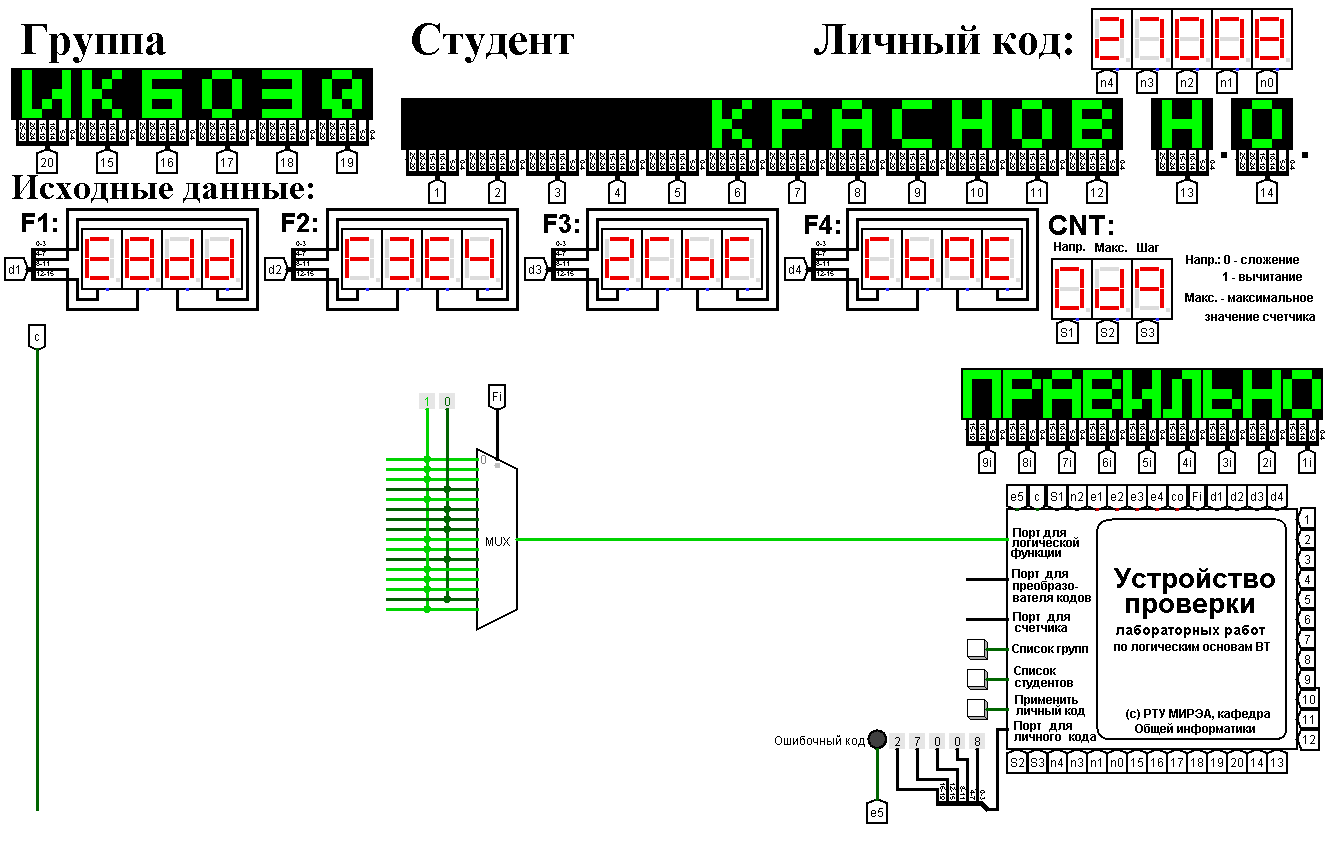
\includegraphics[width=\textwidth]{Мультиплекс 16-1.png}
	\caption{Схема, реализующая логическую функцию при помощи мультиплексора 16-1}
	\label{circ:Мультиплекс 16-1}
\end{figure}

\section{Схема, реализующая логическую функцию при помощи мультиплексора 8-1}	
Реализуем функцию, используя мультиплексор 8-1. Так как мультиплексор 8-1 имеет всего 3 адресных входа, мы не сможем подать на них все 4 логические переменные. Поэтому выберем в качестве адресных переменных три старших логических переменных, а младшую четвертую будем рассматривать наравне с логическими константами как элемент исходных данных для информационных входов.

Пары наборов, на которых значения трех старших переменных <<a>>, <<b>> и <<c>> имеют одинаковые значения, располагаются на соседних строчках таблицы истинности, поэтому можем легко увидеть, как значение переменных для каждой пары наборов будет соотноситься со значением младшей переменной <<d>>. Например, заметим, что при значениях a=0, b=1, c=0 функция зависит от <<$d$>> и равна <<$\bar{d}$>>. Получим таким образом таблицу взаимосвязи значений функции и значений переменной <<d>> (см. табл. \ref{table:Взаимосвязь значений для 8-1}). Таблица \ref{table:Сжатая таблица для 8-1} отображает <<сжатую>> таблицу истинности.

\begin{table}[h!]
	\centering
	\caption{Взаимосвязь значений функции и значений переменной <<d>>}
	\label{table:Взаимосвязь значений для 8-1}
	
\begin{tikzpicture}[remember picture,overlay]
		\foreach \Val\Col in {1/green,2/red,3/blue,4/yellow,5/orange,6/black,7/cyan,8/purple}
			\foreach \Dir in {l,r} {
				\filldraw[
				rounded corners,
				fill=\Col!25!white,
				draw=black!90!\Col,
				thick,
				]
				([shift={(-0.1,0.38)}]pic cs:s\Dir\Val) 
				rectangle 
				([shift={(0.1,-0.15)}]pic cs:e\Dir\Val);
		}
		\foreach \Pos\Func in {1/$F=1$,2/$F=\bar{d}$,3/$F=\bar{d}$,4/$F=0$,5/$F=1$,6/$F=d$,7/$F=1$,8/$F=d$} {
			\node at ([shift={(1.2,0.4)}]pic cs:er\Pos) {\Func};
		}
	\end{tikzpicture}
	
	\begin{tabular}{c|c|c|c|c}
		\textbf{a} & \textbf{b} & \textbf{c} & \textbf{d} & \textbf{F} \\
		\hline
		\tikzmark{sl1}0 & 0 & 0 & \tikzmark{sr1}0 & 1 \\
		\hline
		0 & 0 & 0\tikzmark{el1} & 1 & 1\tikzmark{er1} \\
		\hline
		\tikzmark{sl2}0 & 0 & 1 & \tikzmark{sr2}0 & 1 \\
		\hline
		0 & 0 & 1\tikzmark{el2} & 1 & 0\tikzmark{er2} \\
		\hline
		\tikzmark{sl3}0 & 1 & 0 & \tikzmark{sr3}0 & 1 \\
		\hline
		0 & 1 & 0\tikzmark{el3} & 1 & 0\tikzmark{er3} \\
		\hline
		\tikzmark{sl4}0 & 1 & 1 & \tikzmark{sr4}0 & 0 \\
		\hline
		0 & 1 & 1\tikzmark{el4} & 1 & 0\tikzmark{er4} \\
		\hline
		\tikzmark{sl5}1 & 0 & 0 & \tikzmark{sr5}0 & 1 \\
		\hline
		1 & 0 & 0\tikzmark{el5} & 1 & 1\tikzmark{er5} \\
		\hline
		\tikzmark{sl6}1 & 0 & 1 & \tikzmark{sr6}0 & 0 \\
		\hline
		1 & 0 & 1\tikzmark{el6} & 1 & 1\tikzmark{er6} \\
		\hline
		\tikzmark{sl7}1 & 1 & 0 & \tikzmark{sr7}0 & 1 \\
		\hline
		1 & 1 & 0\tikzmark{el7} & 1 & 1\tikzmark{er7} \\
		\hline
		\tikzmark{sl8}1 & 1 & 1 & \tikzmark{sr8}0 & 0 \\
		\hline
		1 & 1 & 1\tikzmark{el8} & 1 & 1\tikzmark{er8} \\
	\end{tabular}
\end{table}

\begin{table}[h!]
	\centering
	\caption{Сжатая таблица истинности}
	\label{table:Сжатая таблица для 8-1}
	\renewcommand{\arraystretch}{1.5}
	\begin{tabular}{c|c|c|c|c}
		\textbf{a} & \textbf{b} & \textbf{c} & \textbf{F} \\
		\hline
		0 & 0 & 0 & 1 \\
		\hline
		0 & 0 & 1 & $\bar{d}$ \\
		\hline
		0 & 1 & 0 & $\bar{d}$ \\
		\hline
		0 & 1 & 1 & 0 \\
		\hline
		1 & 0 & 0 & 1 \\
		\hline
		1 & 0 & 1 & $d$ \\
		\hline
		1 & 1 & 0 & 1 \\
		\hline
		1 & 1 & 1 & $d$ \\
	\end{tabular}
\end{table}

Теперь, рассматривая переменную <<d>> наравне с константами 0 и 1 в качестве сигналов для информационных входов мультиплексора 8-1, можно по аналогии с предыдущим случаем выполнить реализацию требуемой функции.

Разместим на рабочей области новый мультиплексор, установим ему количество выбирающих (адресных) входов равным трем, и выполним необходимые соединения (рис. \ref{circ:Мультиплекс 8-1}).

\begin{figure}[h!]
	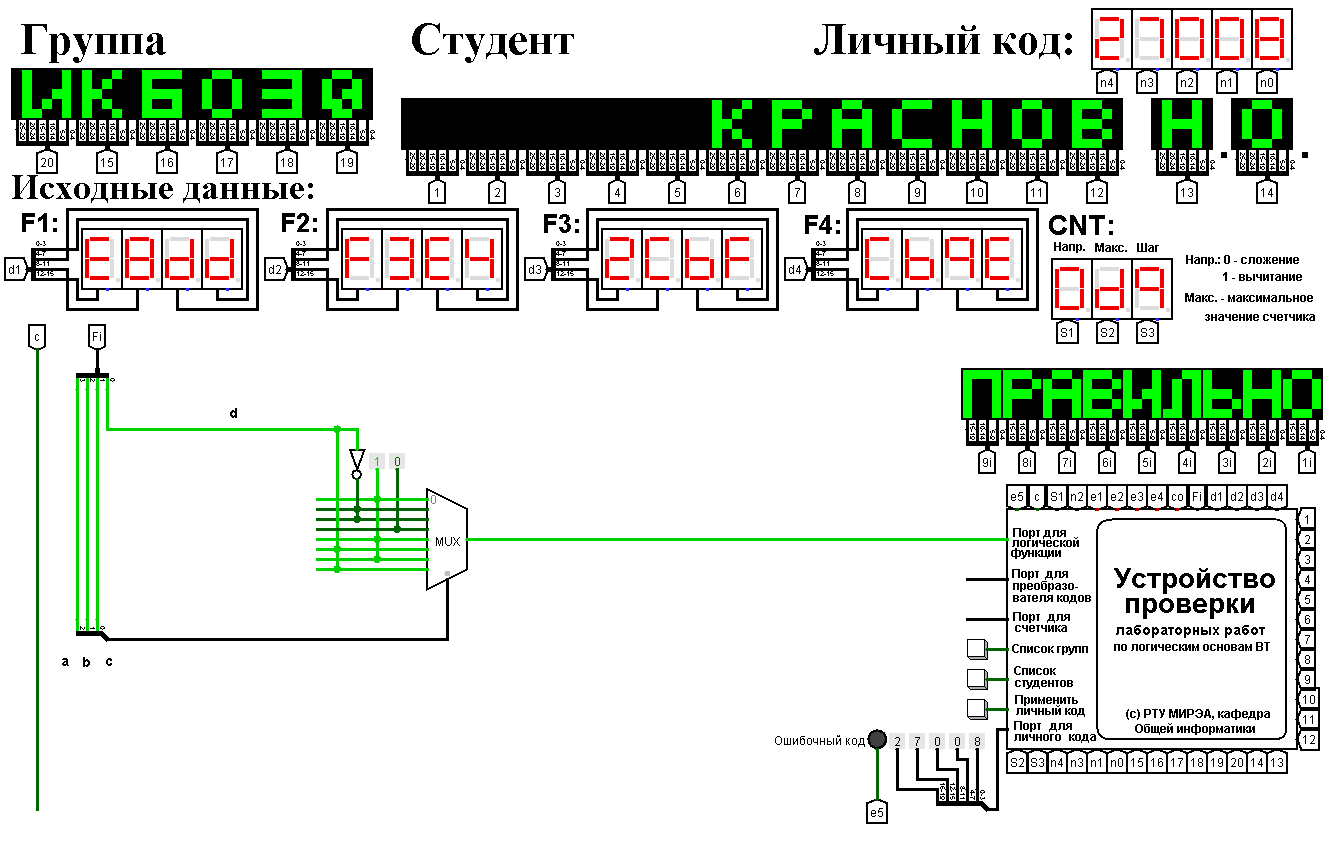
\includegraphics[width=\textwidth]{Мультиплекс 8-1.png}
	\caption{Схема, реализующая логическую функцию при помощи мультиплексора 8-1}
	\label{circ:Мультиплекс 8-1}
\end{figure}

\section{Схема, реализующая логическую функцию при помощи минимального количества мультиплексоров 4-1}
Реализуем функцию, используя минимальное количество мультиплексоров 4-1. Так как мультиплексор 4-1 имеет всего 2 адресных входа, исходную таблицу истинности необходимо будет разбить на 4 фрагмента, причем за реализацию каждого их них будет отвечать отдельный мультиплексор, который мы будем называть операционным. Учтем, что необходимо использовать минимальное количество мультиплексоров 4-1, и постараемся использовать их только там, где это необходимо. Разобьем исходную таблицу истинности на зоны ответственности между операционными мультиплексорами, и посмотрим, можно ли в каком-нибудь из них обойтись без операционного мультиплексора

\begin{table}[h!]
	\centering
	\caption{Взаимосвязь значений функции и значений переменных <<d>> и <<c>>}
	\label{table:Взаимосвязь значений для 4-1}
	
	\begin{tikzpicture}[remember picture,overlay]
		\foreach \Val\Col in {1/green,2/red,3/blue,4/yellow}
		\foreach \Dir in {l,r} {
			\filldraw[
				rounded corners,
				fill=\Col!25!white,
				draw=black!90!\Col,
				thick,
			]
			([shift={(-0.1,0.38)}]pic cs:41s\Dir\Val) 
			rectangle 
			([shift={(0.1,-0.15)}]pic cs:41e\Dir\Val);
		}
		\draw [decorate,decoration={brace,raise=10pt,amplitude=7pt},line width=1pt] ([yshift=4]pic cs:curlystart) -- ([yshift=3]pic cs:curlyend) node [midway,xshift=1.5cm,text width=7cm,rotate=90] {Для каждой зоны необходим операционный мультиплексор};
	\end{tikzpicture}
	
	\begin{tabular}{c|c|c|c|c}
		\textbf{a} & \textbf{b} & \textbf{c} & \textbf{d} & \textbf{F} \\
		\hline
		\tikzmark{41sl1}0 & 0 & \tikzmark{41sr1}0 & 0 & 1\tikzmark{curlystart} \\
		\hline
		0 & 0 & 0 & 1 & 1 \\
		\hline
		0 & 0 & 1 & 0 & 1 \\
		\hline
		0 & 0\tikzmark{41el1} & 1 & 1 & 0\tikzmark{41er1} \\
		\hline
		\tikzmark{41sl2}0 & 1 & \tikzmark{41sr2}0 & 0 & 1 \\
		\hline
		0 & 1 & 0 & 1 & 0 \\
		\hline
		0 & 1 & 1 & 0 & 0 \\
		\hline
		0 & 1\tikzmark{41el2} & 1 & 1 & 0\tikzmark{41er2} \\
		\hline
		\tikzmark{41sl3}1 & 0 & \tikzmark{41sr3}0 & 0 & 1 \\
		\hline
		1 & 0 & 0 & 1 & 1 \\
		\hline
		1 & 0 & 1 & 0 & 0 \\
		\hline
		1 & 0\tikzmark{41el3} & 1 & 1 & 1\tikzmark{41er3} \\
		\hline
		\tikzmark{41sl4}1 & 1 & \tikzmark{41sr4}0 & 0 & 1 \\
		\hline
		1 & 1 & 0 & 1 & 1 \\
		\hline
		1 & 1 & 1 & 0 & 0 \\
		\hline
		1 & 1\tikzmark{41el4} & 1 & 1 & 1\tikzmark{41er4}\tikzmark{curlyend} \\
	\end{tabular}
\end{table}

Из таблицы \ref{table:Взаимосвязь значений для 4-1} видно, что ни на одном из участков не получится обойтись без операционного мультиплексора. Подключим переменные <<a>> и <<b>> к адресным входам управляющего мультиплексора при помощи шины (причем младшая переменная подается на младший адресный вход, а старшая на старший), а к его информационным подключим, в соответствии со сказанным раньше, следующее: к каждому информационному входу управляющего мультиплексора параллельно подключим соответственно каждый из четырех операционных мультиплексоров. К информационным входам подключим константы в соответствии с таблицей \ref{table:Таблица истинности}.

Обратим внимание на то, что последние два фрагмента таблицы являются одинаковыми, поэтому один из них можно не реализовывать. 

Выход управляющего мультиплексора подключим к устройству проверки, и проверим правильности реализации (рис. \ref{circ:Мультиплекс 4-1}).

\begin{figure}[h!]
	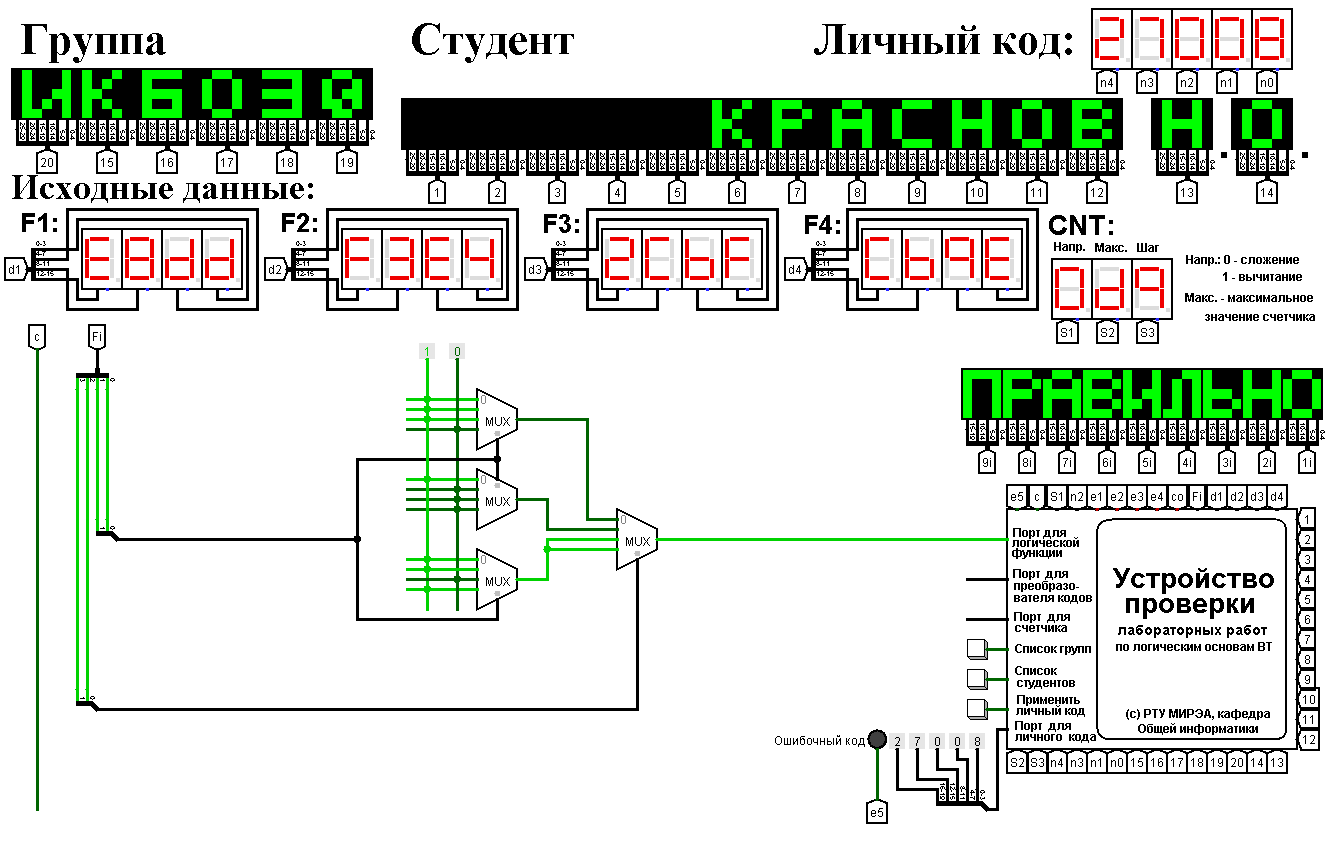
\includegraphics[width=\textwidth]{Мультиплекс 4-1.png}
	\caption{Схема, реализующая логическую функцию при помощи минимального количества мультиплексоров 4-1}
	\label{circ:Мультиплекс 4-1}
\end{figure}

\section{Схема, реализующая логическую функцию при помощи минимального количества мультиплексоров 4-1 и 2-1}
Реализуем функцию, используя минимальное количество мультиплексоров 4-1, 2-1. В качестве отправной точки рассмотрим схему из предыдущего пункта. Попробуем заменить максимальное количество мультиплексоров 4-1 на мультиплексор 2-1. Управляющий мультиплексор заменить не можем, так как у него на входах уникальные сигналы. А вот остальные операционных мультиплексора вполне можно заменить. Из таблицы \ref{table:Взаимосвязь значений для 4-1} выпишем фрагменты, за которые отвечают управляющие мультиплексоры.

\begin{table}[h!]
	\centering
	\caption{Таблица ответственности операционных мультиплексоров в схеме с использованием мультиплексоров 2-1}
	\label{table:Табл. ответственн. 2-1}
	
	
\begin{tikzpicture}[remember picture,overlay]
		\foreach \Val\Col in {1/green,2/red,3/blue,4/yellow} {
			\filldraw[
				rounded corners,
				fill=\Col!25!white,
				draw=black!90!\Col,
				thick,
			]
			([shift={(-0.1,0.38)}]pic cs:21s\Val) 
			rectangle 
			([shift={(0.1,-0.15)}]pic cs:21e\Val);
		}
	\end{tikzpicture}
	
	\begin{tabular}{c|c|c}
		\textbf{c} & \textbf{d} & \textbf{F} \\
		\hline
		\tikzmark{21s1}0 & 0 & 1 \\
		\hline
		0 & 1 & 1 \\
		\hline
		1 & 0 & 1 \\
		\hline
		1 & 1 & 0\tikzmark{21e1} \\
		\hline
		\tikzmark{21s2}0 & 0 & 1 \\
		\hline
		0 & 1 & 0 \\
		\hline
		1 & 0 & 0 \\
		\hline
		1 & 1 & 0\tikzmark{21e2} \\
		\hline
		\tikzmark{21s3}0 & 0 & 1 \\
		\hline
		0 & 1 & 1 \\
		\hline
		1 & 0 & 0 \\
		\hline
		1 & 1 & 1\tikzmark{21e3} \\
		\hline
		\tikzmark{21s4}0 & 0 & 1 \\
		\hline
		0 & 1 & 1 \\
		\hline
		1 & 0 & 0 \\
		\hline
		1 & 1 & 1\tikzmark{21e4} \\
	\end{tabular}
\end{table}

Как видно на примере зеленого фрагмента в таблице \ref{table:Табл. ответственн. 2-1}, отвечающего за значения одного из операционных мультиплексоров, при подаче на вход <<c>>=0 -- на выходе всегда будет константное значение 1, при подаче на вход <<c>>=1 -- на выход всегда будет значение $\bar{d}$. По такому же принципу упростим все оставшиеся фрагменты таблицы, получив схему, показанную на рис. \ref{circ:Мультиплекс 2-1}.

Учтем, что последний фрагмент таблицы \ref{table:Табл. ответственн. 2-1} повторяет предыдущий, поэтому повторно его можно не реализовывать.

\begin{figure}[h!]
	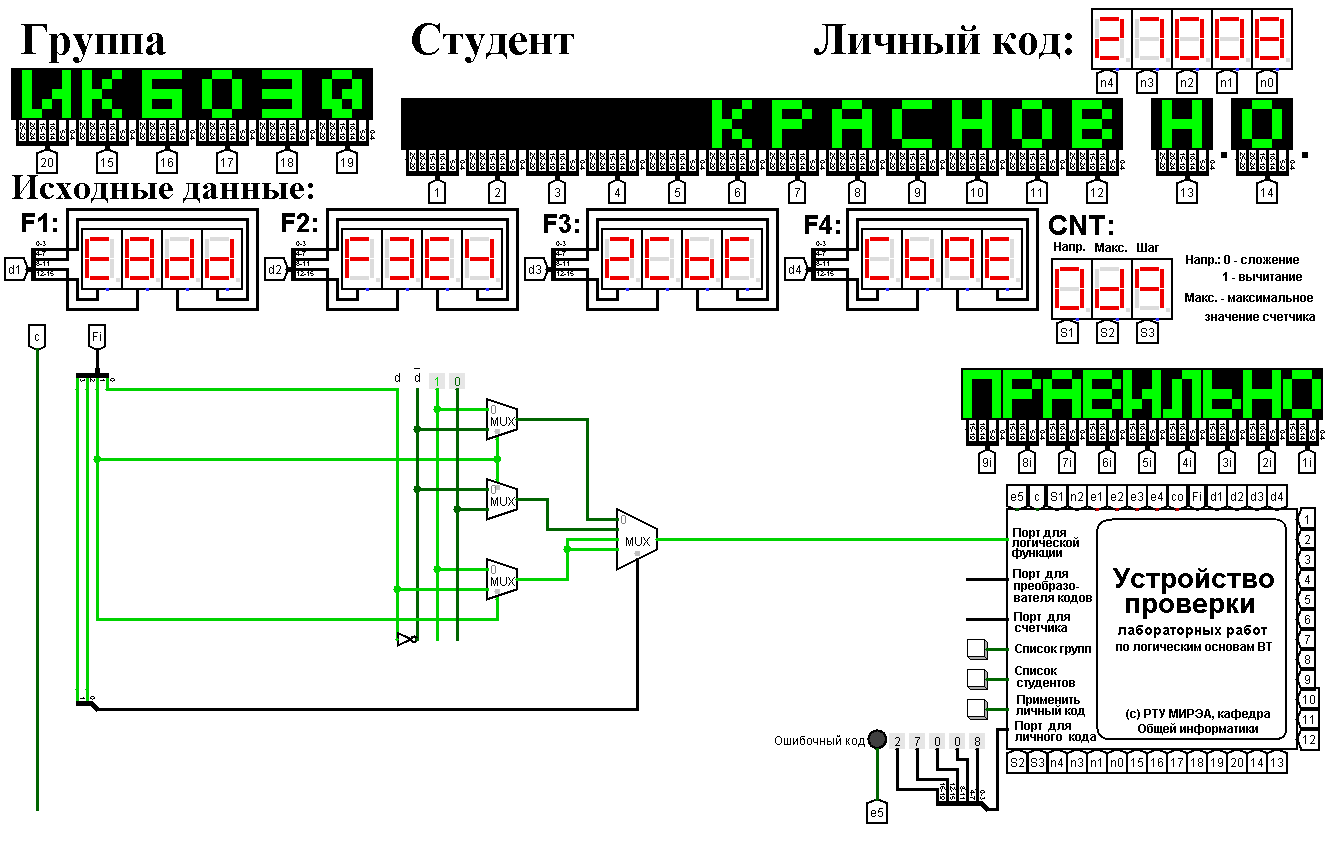
\includegraphics[width=\textwidth]{Мультиплекс 2-1.png}
	\caption{Схема, реализующая логическую функцию при помощи минимального количества мультиплексоров 4-1 и 2-1}
	\label{circ:Мультиплекс 2-1}
\end{figure}

\chapter{ВЫВОДЫ}
В ходе работы была восстановлена таблица истинности от четырех переменных в реализации мультиплексоров разными способами, а именно: мультиплексор 16-1, мультиплексор 8-1, минимальное количество мультиплексоров 4-1, минимальная комбинация мультиплексоров 4-1 и 2-1. После реализации каждого из четырех способа, работа схем была протестирована и все схемы оказались верными.
	
\begin{thebibliography}{99}
	\bibitem{Методичка}
	\textbf{Смирнов, С.С.} Информатика. Методические указания по выполнению практических работ / С.С. Смирнов, Д.А. Карпов. – Москва, МИРЭА – Российский технологический университет, 2020. – 102 с.
	
	\bibitem{Logisim}
	Logisim / разработчик: Карл Бурч. – 2014. – URL: http://www.cburch.com/logisim/index.html (дата обращения 26.10.2022). – версия 2.7.0 . – Электронная программа : электронная.
\end{thebibliography}
	
	
\end{document}
